\section{Mutable types}
\subsection{Lists}

\begin{frame}[fragile]
    \frametitle{List: definition}
    A list is an \emph{ordered} sequence of elements, which are \emph{not necessarily of the same type} and are accessible via a unique \emph{index} (integer), which is the element's position within the list.
   
    \vspace{1em}
        \begin{center}
    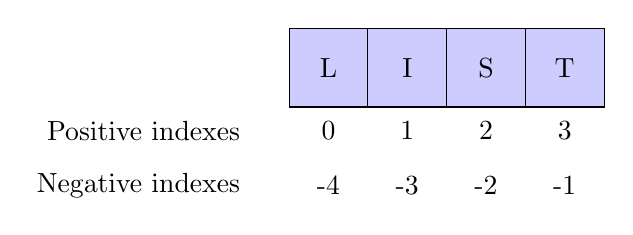
\begin{tikzpicture}
        \filldraw[step=1.0,black, thin, fill=blue!20] (0., 0. ) grid (4, 1) rectangle(0, 0);
        \draw (0.5, 0.5 ) node {L};
        \draw (1.5, 0.5 ) node {I};
        \draw (2.5, 0.5 ) node {S};
        \draw (3.5, 0.5 ) node {T};
        
        \def\wpos{-0.3}
        \def\wneg{-1}
        \def\lab{-0.5}

        \draw (0.5, \wpos ) node {0};
        \draw (1.5, \wpos ) node {1};
        \draw (2.5, \wpos ) node {2};
        \draw (3.5, \wpos ) node {3};
        \draw (\lab, \wpos ) node [anchor=east, align=right]{Positive indexes};
        
        \draw (0.5, \wneg ) node {-4};
        \draw (1.5, \wneg ) node {-3};
        \draw (2.5, \wneg ) node {-2};
        \draw (3.5, \wneg ) node {-1};
        \draw (\lab, \wneg ) node [anchor=east, align=right]{Negative indexes};
    \end{tikzpicture}
    \end{center}



    \begin{block}{Tuples}
        Python \verb+tuple+ can be viewed as immutable list. \verb+[]+ are replaced by \verb+()+
    \end{block}

\end{frame}

\begin{frame}[fragile]
    \frametitle{List: usage}
    
    Lists are used: 
    \begin{itemize}
        \item{The script arguments are stored in a list of strings (\verb+sys.argv+)}
        \item{The Python path is stored in a list (\verb+sys.path+)}
        \item{Used in loops (repeat operations over a list of objects)}
        \item{The \verb+dir+ function returns methods/attributes as a list of string}
        \item{Might be used as \emph{stacks} (last-in, first-out)}
        \item{\item{To handle function arguments (\verb+*args+ arguments)}}
    \end{itemize}

    \begin{block}{Note}
        Lists are not optimized for first-in, first-out treatments (\href{https://docs.python.org/fr/3/tutorial/datastructures.html}{python.org})
    \end{block}
\end{frame}

\begin{frame}[fragile]
    \frametitle{List: manipulation}
    Open the \verb+list.py+ file and let's play with lists!

    \begin{block}{More about lists}
        To have more about lists, visit \href{https://docs.python.org/3/tutorial/datastructures.html#more-on-lists}{python.org}
    \end{block}

\end{frame}

